% !TEX root = ../thesis-example.tex
%
\chapter{Robot Cartesian Control}
\label{sec:concepts}

\cleanchapterquote{Vogliamo, per esempio, prendere una sigaretta. Il nostro movimento viene regolato istante per istante dal valore dell'incompiutezza dell'azione.}{Norbert Wiener}{La Cibernetica}
\let\thefootnote\relax\footnotetext{This chapter is based on the works published in \cite{RocchiMingoHoffman:15} and revised in \textbf{INSERIRE EVENTUALI ALTRI PAPERS}}

In this chapter a new whole body motion library, called \textbf{OpenSoT}, is presented. \textbf{OpenSoT} implements the idea of decoupling atomic tasks/constraints descriptions and solvers to execute multiple tasks and achieve complex motion behaviors. It employs a solver implementing a cascade of Quadratic Programming (QP) problems, and a set of tasks and constraints in velocity space in order to solve a generic hierarchical inverse kinematics problem on a humanoid robot. Furthermore a robust IK solver is presented. It is based on a state machine that hides all the complexity of the underneath QP solver. The IK solver make use of a state-of-art library in QP resolution using the active set approach: \emph{qpOASES} \cite{Ferreau:14}. 
\textbf{OpenSoT} has been used in the DRC Finals, by the WALK-MAN team, to perform all the manipulation tasks involving \emph{whole-body} motion while taking into account constraints that are fundamental when working with real hardware. During the developing period, the \textbf{OpenSoT} framework allowed the fast evaluation of different solutions for the same high-level task reformulating the IK Problem without changing the IK solver structure. 

Typical methods and techniques to map task-space commands to joint commands can be classified as inverse kinematics or inverse dynamics schemes and can be implemented using a variety of low level controllers. \textbf{OpenSoT} belongs in the first group: the goal was therefore to develop a high performance and flexible library that can generate reliably complex and efficient motions at whole body level. This yields the following features that make the implementation of \textbf{OpenSoT} unique and attractive:   
\begin{itemize}
\item Demonstrates adequate modularity through the separation of task descriptions, control schemes and solvers maximizing customization, flexibility and expandability.  
\item Provides user friendly interfaces for defining tasks, constraints and solvers to promote integration and cooperation in the emerging field of whole-body hierarchical control schemes.
\item Demonstrates computation efficiency to allow for real time performance implementations.
\item Allows ease of use and application with arbitrary robots through the Universal and Semantic Robotic Description Formats (URDF and SRDF).
\end{itemize}

The chapter is structured as follows. Section \hyperref[sec:robot-Cartesian-control:related-works]{\textbf{Related Works}} introduces the related literature on Whole-Body Inverse Kinematics/Dynamics compliant control, focusing mainly on schemes actually used in real hardware. In section \hyperref[sec:robot-Cartesian-control:inverse-kinematics]{\textbf{Inverse Kinematics}} the basics concepts of inverse kinematics are introduced as well as different methods to solve it.
Section \hyperref[sec:robot-Cartesian-control:opensot]{\textbf{OpenSoT}} describes the library. Section \hyperref[sec:robot-Cartesian-control:experiments]{\textbf{Experiments}} shows some results regarding the use of the \textbf{OpenSoT} library.

\section{Related Works}
\label{sec:robot-Cartesian-control:related-works}
Kinematic and dynamic inversion are well known problems in robotics. In general, given some tasks specified in Cartesian position, velocity, accelerations or forces, we want to find the joints positions, velocities, accelerations or torques that realize those tasks. Many solutions to this problem have been presented for single and multiple kinematic chains \cite{Siciliano:90} and \cite{Wensing:13}. An interesting subset of these algorithms are those based on numerical optimization, since they allow for the explicit introduction of unilateral/bilateral constraints in the inverse kinematic/dynamic problem, which are fundamental when working on the real robotic hardware \cite{Escande:12}.

In this brief review of the state of the art on full-body control, the focus will be on some of the recent frameworks that have been used successfully on humanoid robots. One of the most famous framework oriented to whole-body control is the Stack of Tasks (SoT) from LAAS \cite{Mansard:09}. This work can be categorized under the group of the IK solvers with different implementations allowing to use both the classical pseudoinverse approach with null-space projection or decomposition methods that allow for one-shot solving of the whole stack (HCOD), to enforce lexycographic order in the stack. SoT has been used mostly in HRP-2 platform and part of the presented work is inspired by this one. 
Another framework for whole-body task specification and control is iTaSC \cite{Smits:09},  with the current implementation supporting velocity-based whole-body control and equality constraints. It has been successfully demonstrated on the PR2 robot.
In \cite{Fallon:14} IK is solved using a nonlinear program. Two kind of nonlinear optimizations are set up: a single-shot IK and trajectory optimization. This work was used in Atlas during the DRC trials coupled with a position control.
A nonlinear optimization is also performed in \cite{Pattacini:10} to perform IK on the iCub platform.
There are many other frameworks including those that are based on Inverse Dynamics, implemented on top of a pure low level torque control (a notable example is \cite{Sentis:10}), yet it is difficult to find hardware platforms mature enough to implement control schemes of such frameworks and up to now no complex tasks have been experimentally demonstrated yet in humanoid bipedal robots.


\section{Inverse Kinematics}
\label{sec:robot-Cartesian-control:inverse-kinematics}
The \textbf{Inverse Kinematics Problem} consists of the determination of the joint variables corresponding to a given task for the end-effector in \textbf{Operational Space}. The IK Problem is in general highly non-linear (a closed form solution may not be available) and may have multiple solutions. In particular, if the robot is \textbf{redundant} for the task, the IK Problem has an infinite number of solutions. A solution may be not admissible due to the manipulator kinematics structure (for example joint limits). The existence of solutions is guaranteed if the given goal in the operation space belongs to the manipulator \textbf{dexterous space}.

Despite the relationship between joint position variables and operational space poses is not linear, the mapping between joint velocity variables and operational space velocities is linear through the Jacobian matrix:
\begin{equation}
    \label{differential_kineamtics}
    \mathbf{v} = \mathbf{J}(\mathbf{q})\mathbf{\dot{q}}
\end{equation}
where the Jacobian (we will skip the dependency on the actual configuration $\mathbf{q}$ from now on) is expressed from a certain \emph{base link} to a certain \emph{distal link}, and operational space velocities of the \emph{distal link} are expressed in the \emph{base link} reference frame.
A general solution, for the redundant case, of (\ref{differential_kineamtics}) is:
\begin{equation}
    \label{differential_inverse_kineamtics}
    \mathbf{\dot{q}}_d = \mathbf{J}^{\dagger}\mathbf{v}_d + \left( \mathbf{I} - \mathbf{J}^{\dagger}\mathbf{J} \right)\mathbf{\dot{q}}_0
\end{equation}
where $\mathbf{J}^{\dagger}$ is the \emph{pseudo inverse} of the Jacobian and $\dot{\mathbf{q}}_0$ is an arbitrary joint space velocity. 
This solution allows also \emph{task prioritization}: 
\begin{equation}
    \label{another_task}
\mathbf{\dot{q}}_0 = \mathbf{J}_0^{\dagger}\mathbf{v}_0
\end{equation}
in particular, the solution given by (\ref{differential_inverse_kineamtics}) with (\ref{another_task}), project the joint velocities of the second task onto the null space of the first task removing all the components that would interfere with it \cite{SicilianoKathib:08}. Many other solutions of (\ref{differential_kineamtics}) are available in literature \cite{Siciliano:91}, \cite{Flacco:14}. Singularities in the Jacobian, as well as joint velocity limits, are often handled with the \emph{Singularity Robust Inverse} (SRI) \cite{Nakamura:90}, \cite{Maciejewski:89}.
The problem of such schemes is that they do not handle constraints in the form of inequalities. 

Another way to see the inverse problem of (\ref{differential_kineamtics}) is to consider it as a Quadratic Programming (QP) problem with linear constraints:
\begin{equation} 
\label{optimization_problem}
\begin{array}{c}
\mathbf{\dot{q}}_d = \underset{\mathbf{\dot{q}}}{\operatorname{argmin}} \ \Arrowvert \mathbf{J} \mathbf{\dot{q}}-\mathbf{v}_d \Arrowvert\\
s.t. \ \mathbf{A}\mathbf{\dot{q}} \leq \mathbf{b}
\end{array}
\end{equation}
where: 
\begin{equation}
    \Arrowvert \mathbf{J} \mathbf{\dot{q}}-\mathbf{v}_d \Arrowvert = \mathbf{\dot{q}}^\text{T}\mathbf{J}^\text{T}\mathbf{J}\mathbf{\dot{q}} - 2(\mathbf{J}\mathbf{\dot{q}})^\text{T}\mathbf{v}_d+\mathbf{v}_d'\mathbf{v}_d
\end{equation}
is the quadratic cost function that is minimized and 
\begin{equation}
    \mathbf{A}\mathbf{\dot{q}} \leq \mathbf{b}
\end{equation}
is a general linear constraint. There exist basically two big families of methods to solve the problem in (\ref{optimization_problem}); \emph{active set} and \emph{interior point} methods. 

\textbf{Active set} methods consider the constraints, as equalities, only when active so that the problem (\ref{optimization_problem}) is transformed in a QP with only equalities. At each iteration the new active set is computed checking for the infeasible constraints.

\textbf{Interior point} methods use barrier functions (most of the time $log$ functions) to penalize the cost function in the region where the bounds are violated and the solution is found to iteratively relaxing the barrier function.

Even under the optimization point of view, the task prioritization can be handled considering the minimization of the cost function under equality constraints given by the minimization of previous tasks. This technique is commonly referred as \emph{Stack of Tasks} (SoT) \cite{Mansard:09}. 

The presented work is based on the SoT technique to derive the IK Problem and on the active set method to solve the relative optimization problem. 



\section{OpenSoT}
\label{sec:robot-Cartesian-control:opensot}
\textbf{OpenSoT} is a robotics library tool oriented to Whole-Body Control. The main idea behind its implementation is to decouple the task description, and the solver used to solve the general Inverse Kinematics/Dynamics problem. This distinction allows to easily switch the control, even with the same task description, by using a different solver. \textbf{OpenSoT} aims at providing a standard way to describe the aforementioned entities in an atomic way, and at the same time to build a repository of common entities that can be reused to create a generic stack using a user friendly development and integration interface.

\textbf{OpenSoT} is based on three main entities:
\begin{description}
    \item[Robot Model] is an object that contains all the kinematics/dynamics characteristics of the robot, as well as links in contact with the environment and other information
    \item[IK Problem] is the set of tasks, constraints and bounds. Each of them require the robot model to be instantiated
    \item[Solver] that takes the IK Problem in input and gives the new values of the controlled variable in output
\end{description}
Each of these entities needs to be updated at each step of the control loop with new values coming from the sensors (joint positions, joint velocities, forces/torques at FT sensor and so on). 

\subsection{Robot Model}
\label{sec:robot-Cartesian-control:opensot:sec:robot-model}
The robot model library (called \textbf{idynutils}) is in charge to perform forward kinematics and inverse dynamics, updating the \emph{world} pose considering the kinematics and the sensors of the robot, handling links in contact, compute CoM kinematics and dynamics and so on . It basically takes in input a URDF and a SRDF of the robot in order to generate all the data structure needed. 

The \emph{world} reference frame is the frame wrt all the Jacobians are computed. The \emph{world} frame can be connected to any link of the robot called \emph{anchor} link. During the update procedure, tha user can decide or not to update the \emph{world}, in the first case we are considering a fixed base robot, in the second we consider a floating base robot. The user can also update the \emph{world} considering sensors measurement such as the IMU. Finally, the user can directly provide the pose of the \emph{world} computed by an external library.

At every control loop, the robot model needs to be updated with measured joint position, velocities, F/T sensors values and list of the links that are in contact with the environment. The \textbf{idynutils} library is downloadable at the url: \url{https://github.com/robotology-playground/idynutils}. 

\subsection{IK Problem}
The IK Problem consists in the set of tasks, constraints and bounds that have to be considered in order to solve an high level task. For instance, the robot may have to turn a valve while keeping balance and without reach the joint limits. \textbf{OpenSoT} allows the user to choose between a library of tasks, constraints and bounds or provides bases classes to write new tasks, constraints and bounds. 

When a new IK Problem is written, \textbf{tasks} can be organized considering \emph{soft} or \emph{hard} priorities. Tasks are in \emph{soft} priority when the Jacobians are \emph{stacked}:
\begin{equation}
\mathbf{J} = \begin{bmatrix}
\mathbf{J}_1\\ 
\mathbf{J}_2
\end{bmatrix}
\end{equation}
and the related cost function became:
\begin{equation}
\Arrowvert \mathbf{J} \mathbf{\dot{q}}-\mathbf{v}_d \Arrowvert = \Arrowvert \mathbf{J}_1 \mathbf{\dot{q}}-\mathbf{v}_{d,1} \Arrowvert_{W_1} + \Arrowvert \mathbf{J}_2 \mathbf{\dot{q}}-\mathbf{v}_{d,2} \Arrowvert_{W_2}
\end{equation}
where $W_1$ and $W_2$ are positive definite gain matrices that permits to define the \emph{soft} priority between the tasks. In this situation the tasks may interfere each other.
Tasks are in \emph{hard} priority when the lowest priority task is projected in the null space of high priority task, as in \ref{differential_inverse_kineamtics}. In this latter case the high priority task is always (if possible) accomplished. \textbf{OpenSoT} permits to define mixed \emph{hard} and \emph{soft} priorities when describing the IK Problem. 

\textbf{Constraints} can be divided in \emph{local} and \emph{global} constraints. The first can be associated just to a particular task and are not apply to all the tasks that are in low priority, for instance bounds on the pose of the end effector are \emph{local} constraints. \emph{Global} constraints are applied to all the tasks, for instance self collision avoidance. A constraint is \emph{local} or \emph{global} depending on which tasks are performed: let consider a task $\mathbf{J} \in \mathbf{R}^{m\times n}$ with $rank(\mathbf{J}) = m$ and let consider a constraint $\mathbf{A}\mathbf{\dot{q}} \leq \mathbf{b}$, if 
\begin{equation}
rank\left ( \begin{bmatrix}
\mathbf{J}\\ 
\mathbf{A}
\end{bmatrix} \right ) = m
\end{equation}
then $\mathbf{A}$ is a \emph{local} constraint and is not needed to specify it in all the low priority tasks (check Appendix \ref{app:local-constr} for the proof).

\textbf{Bounds} are constraints where $\mathbf{A} = \mathbf{I} \in \mathbf{R}^{n\times n}$ where $n$ is the number of variables (joints) of the problem. Therefore bounds are considered always as global constraints.

\subsubsection{Implemented Tasks, Constraints and Bounds}
Each task is defined by:
\begin{equation}
    T = \left[ \mathbf{J}, \quad \mathbf{v} \right]
\end{equation}
where $\mathbf{J}$ is the Jacobian of the task and $\mathbf{v}$ is the task reference. \textbf{Cartesian tasks} Jacobians and references are defined as:
\begin{equation}
\begin{matrix}
\mathbf{J} = {^\text{b}\mathbf{J}^\text{l}_\text{ee}} \\ 
\mathbf{v} = {^\text{b}\mathbf{v}_\text{ee}}
\end{matrix}
\end{equation}
where $b$ is the base where the velocities are expressed, $l$ is the first link of the kinematic chain taken in consideration and $ee$ is the end-effector. Is worth to notice that is possible to take in consideration a sub-set of joints in the Jacobian (setting to zero the columns not needed) as well as directions (cutting the rows not needed). The velocity reference is computed as (apices are omitted):
\begin{equation}
\mathbf{v} = \begin{bmatrix}
\mathbf{\dot{p}_d}  \ + \ K_p\mathbf{e_p}\\ 
\mathbf{w_d}  \ + \ K_o\mathbf{e_o}
\end{bmatrix}
\end{equation}
and
\begin{equation}
\begin{array}{l}
\mathbf{e_p} = \mathbf{p_d} - \mathbf{p}
\\
\\
\mathbf{e_o} = -(\eta_d \boldsymbol{\epsilon} - \eta \boldsymbol{\epsilon_d} + [\boldsymbol{\epsilon_d}\times] \boldsymbol{\epsilon})
\label{cartesian_error}
\end{array}
\end{equation}
where $\mathbf{p_d}$ is the desired position and $\boldsymbol{\alpha_d} = [\eta_d \quad \boldsymbol{\epsilon}]$ is the desired orientation expressed as a quaternion \cite{Nakanishi:08}, $K_p$ and $K_o$ are positive definite matrices and $\mathbf{\dot{p}_d}$ and $\mathbf{w_d}$ are the desired Cartesian velocity for the end-effector.
A particular case is the \textbf{CoM} task which is defined as a Cartesian position task. The CoM Jacobian is defined as:
\begin{equation}
\mathbf{J_\text{CoM}} = \frac{\sum_{i=0}^{n} m_i\mathbf{J_{\textbf{CoG,i}}}}{\sum_{i=0}^{n} m_i}
\end{equation}
where $\mathbf{J_{\textbf{CoG,i}}}$ is the Jacobian of the $ith$ Center of Gravity link.
\textbf{Force Control} can be achieved at the velocity level using admittance control:
\begin{equation}
\Delta\mathbf{p} = C \left({^\text{b}\mathbf{f}_\text{d,ee}} - {^\text{b}\mathbf{f}_\text{m,ee}} \right )
\end{equation}
and 
\begin{equation}
{^\text{b}\mathbf{f}_\text{m,ee}} = \begin{bmatrix}
{^\text{b}\mathbf{R}_\text{ft}} & \mathbf{0}\\ 
\mathbf{0} & {^\text{b}\mathbf{R}_\text{ft}} 
\end{bmatrix}
\begin{bmatrix}
\mathbf{I} & \mathbf{0}\\ 
{^\text{ee}\mathbf{p}_\text{ft}\times} & \mathbf{I} 
\end{bmatrix}{^\text{ft}\mathbf{f}_\text{m,ft}}
\end{equation}
where ${^\text{b}\mathbf{f}_\text{d,ee}}$ is the desired wrench that the robot has to exert to the environment, ${^\text{ft}\mathbf{f}_\text{m,ft}}$ is the wrench that the robot is exerting to the environment measured on the force/torque sensor, ${^\text{b}\mathbf{R}_\text{ft}}$ is the rotation from the base link to the force/torque reference frame, ${^\text{ee}\mathbf{p}_\text{ft}\times}$ is the skew symmetric matrix computed from the distance between the force/torque reference frame and the end-effector reference frame, $C$ is a positive definite compliance matrix. The computed $\Delta\mathbf{p}$ is then used to set a new reference for a Cartesian Task.
\textbf{Joint space tasks} Jacobians and references are defined as:
\begin{equation}
\begin{matrix}
\mathbf{J} = \mathbf{I} \\ 
\mathbf{v} = \mathbf{g(q)}
\end{matrix}
\end{equation}
where $\mathbf{I}$ is the identity matrix and $\mathbf{g(q)}$ is a function in joint space. A classical joint space task is the \textbf{Postural Task} defined as:
\begin{equation}
\mathbf{v} = \frac{\mathbf{q}_\text{d} - \mathbf{q}}{\Delta T}
\end{equation}
or \textbf{Acceleration Norm Minimization} at the velocity level \cite{Flacco:15}:
\begin{equation}
\mathbf{v} = \mathbf{\dot{q}}_\text{prev}
\end{equation}
where the reference is the previous desired joint velocity.
Through joint space tasks is possible to have non-linear references functions using the gradient:
\begin{equation}
\mathbf{v} = \nabla \mathbf{g(\mathbf{q})}
\end{equation}
Using this technique many joint space tasks have been implemented such as \textbf{Minimum Effort} \cite{RocchiMingoHoffman:15} and \textbf{Manipulability Optimization} \cite{Nakamura:90}. 

Constraints are defined as:
\begin{equation}
    C = \left[ \mathbf{A}, \quad \mathbf{b}_\text{min}, \quad \mathbf{b}_\text{max} \right]
\end{equation}
where $\mathbf{A}$ is the constraint matrix and $\mathbf{b}_\text{min}$ and $\mathbf{b}_\text{max}$ are the lower and upper constraints. The \textbf{Self Collision Avoidance} constraint is fundamental during real task execution. The basic idea is to calculate the minimum distance between every link pair in every control loop and obtain a list of several closest link pairs according to these minimum distances. For each of these link pairs of interest, we try to control the relative velocity of the one link  with respect to the other in the direction connecting the closest points on the two links respectively, which is called velocity damping. To accelerate the computation of minimum distance of each link pair, capsule, sphere-swept  line, is chosen. 
\begin{figure}
  \centering
    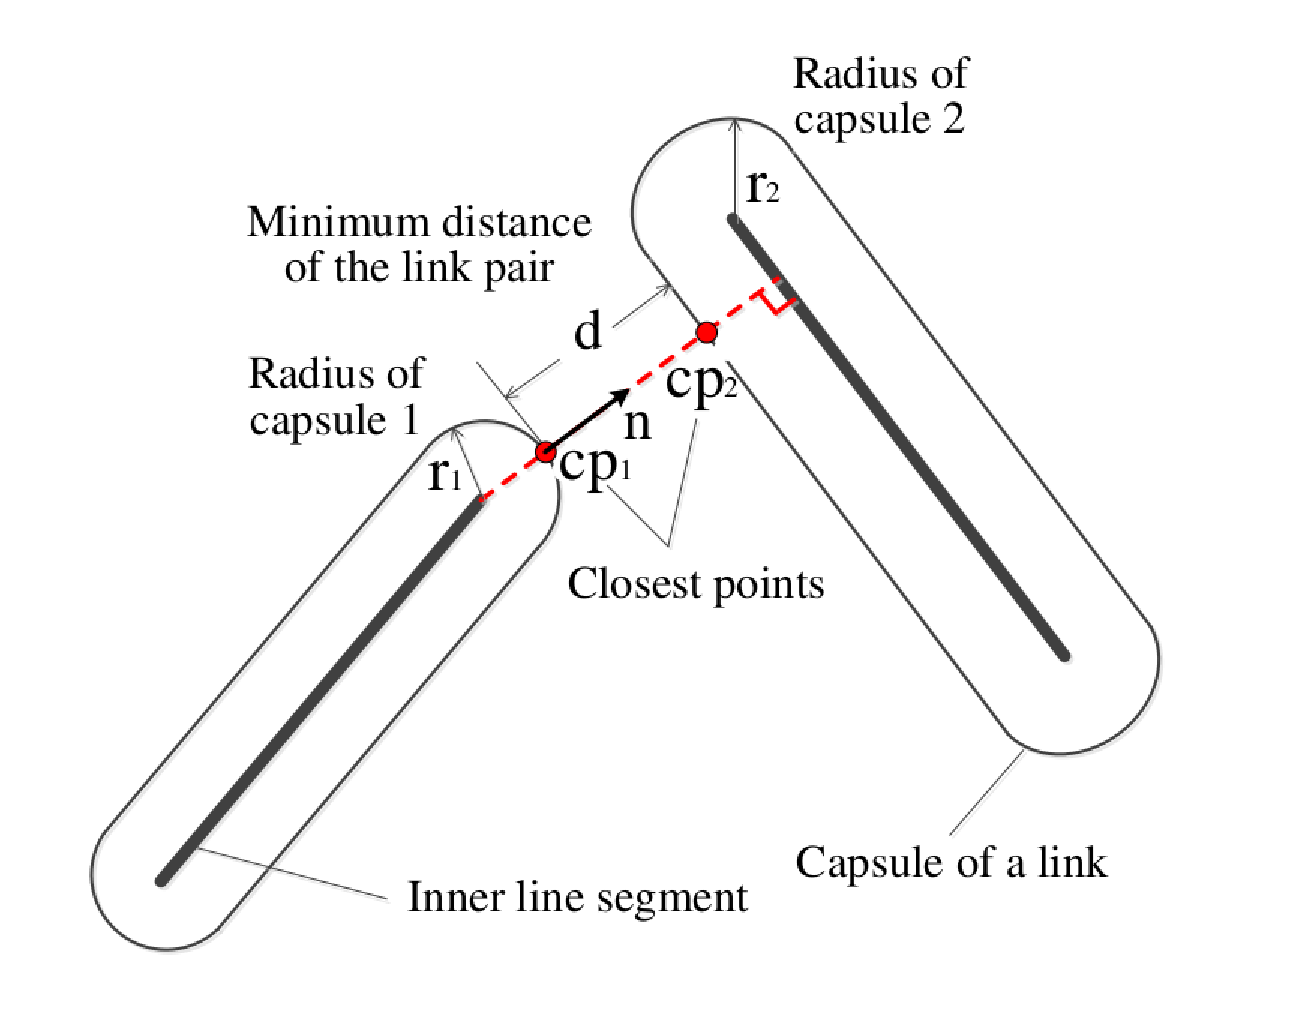
\includegraphics[width=0.7\textwidth]{gfx/link_pair}
    \vspace{-50pt}
    \caption{Schematic diagram of the collision avoidance constraint on a capsule pair representing the collision model for a link pair}\label{link_pair}
\end{figure}
the minimum distance between a capsule pair and the shortest points on them can be easily obtained by using the Flexible Collision Library (FCL) \cite{Pan:12}. Once the closest points are computed, for instance, $ \mathbf{cp}_1 $ and $ \mathbf{cp}_2 $, the relative motion of the capsule pair is going to be restricted in the direction:

\begin{equation} 
\label{eq:unit_vector}
\begin{array}{c}
\mathbf{n} = \dfrac{\mathbf{cp}_2-\mathbf{cp}_1}{\Arrowvert \mathbf{cp}_2-\mathbf{cp}_1 \Arrowvert} 
\end{array}
\end{equation}

Where the distance $ \Arrowvert \mathbf{cp}_2-\mathbf{cp}_1 \Arrowvert $ is calculated according to the Euclidean L2-norm. So, the relative velocity constraint in this direction can be formulated as follows:

\begin{equation} 
\label{eq:SCA_constraint}
\begin{array}{c}
\mathbf{n}^{T}[\mathbf{J}(\mathbf{cp}_1,\mathbf{q})-\mathbf{J}(\mathbf{cp}_2,\mathbf{q})]\dot{\mathbf{q}} \leq \varepsilon \dfrac{d-d_s}{\Delta t} 
\end{array}
\end{equation}
The \textbf{Robot Dynamics} is another fundamental constraint since it filter all the motions that are not dynamically feasible for the robot according to the maximum and minimum allowed joint torques. The dynamics of the robot can be written as:
\begin{equation}
\mathbf{M}(\mathbf{q})\mathbf{\ddot{q}} + \mathbf{C}(\mathbf{q},\mathbf{\dot{q}})\mathbf{\dot{q}} + \mathbf{G}(\mathbf{q}) = \boldsymbol{\tau} - \mathbf{J}^T_c\mathbf{f}_c
\end{equation}
where $\mathbf{M}(\mathbf{q})$ is the joint space inertia matrix, $\mathbf{C}(\mathbf{q},\mathbf{\dot{q}})$ takes into account about centrifugal and Coriolis terms, $\mathbf{G}(\mathbf{q})$ are the gravity torques, $\boldsymbol{\tau}$ are the joint torques and $\mathbf{J}^T_c\mathbf{f}_c$ are the torques due to contacts. Considering an acceleration level control and considering that each joint can provide $\left[\tau_{\text{i,min}}, \ \tau_{\text{i,max}} \right]$, is possible to write the constraint as:
\begin{equation}
\mathbf{D}(\mathbf{q, \dot{q}}) + \boldsymbol{\tau}_\text{min}\leq \mathbf{M}(\mathbf{q})\mathbf{\ddot{q}} \leq  \mathbf{D}(\mathbf{q, \dot{q}}) + \boldsymbol{\tau}_\text{max}
\end{equation}
with $\mathbf{D}(\mathbf{q, \dot{q}},\mathbf{f}_c) = -\left(\mathbf{C}(\mathbf{q},\mathbf{\dot{q}})\mathbf{\dot{q}} + \mathbf{G}(\mathbf{q}) - \mathbf{J}^T_c\mathbf{f}_c \right )$. Is then possible to approximate the joint acceleration $\mathbf{\ddot{q}}$ as:
\begin{equation}
\mathbf{\ddot{q}} = \frac{\mathbf{\dot{q}}-\mathbf{\dot{q}}_\text{prev}}{\Delta T}
\end{equation}
the constraint can be rewritten as:
\begin{equation}
\Delta T \left(\mathbf{D}(\mathbf{q}, \mathbf{\dot{q}}) + \boldsymbol{\tau}_\text{min}\right ) + \mathbf{M}(\mathbf{q})\mathbf{\dot{q}}_\text{prev} \leq
\mathbf{M}(\mathbf{q})\mathbf{\dot{q}} 
\leq  \Delta T \left(\mathbf{D}(\mathbf{q}, \mathbf{\dot{q}}) + \boldsymbol{\tau}_\text{max}\right)+ \mathbf{M}(\mathbf{q})\mathbf{\dot{q}}_\text{prev}
\label{robot_dynamics_constraint}
\end{equation}
Other constraints have been implemented inside \textbf{OpenSoT} such as \textbf{Static Stability} (CoM has to lies inside the support polygon), \textbf{CoM Velocity} and so on. 

Finally bounds are defined as:
\begin{equation}
    C = \left[ \mathbf{u}_\text{min}, \quad \mathbf{u}_\text{max} \right]
\end{equation}
Typical bounds are \textbf{Joint Limits} avoidance and \textbf{Joint velocity limits} avoidance \cite{RocchiMingoHoffman:15}. For all the tasks, constraints and bounds implemented in \textbf{OpenSoT} please refers to the website \url{https://github.com/robotology-playground/OpenSoT}.
 
\subsection{Solver}
In \textbf{OpenSoT} a solver is an object that permits to minimize a certain cost function $f(x)$. The solver may or not take into account constraints, bounds and priorities. Anyway, the IK step is potentially dangerous for the robot for different reasons that depend largely on the algorithm chosen to solve the IK problem.
For this reasons, in the default solver provided with \textbf{OpenSoT}, some characteristics are provided to be considered \emph{robust} in the real task execution scenario: \emph{singularity robustness} and \emph{constraints/bounds handling}.
The first one is required anytime the robot is near the kinematics singularities and the algorithm has to assure that no high joint velocities are generated.
The latter is fundamental to prevent a task from potentially damaging the robot. 

Considering these requirements, the presented IK solver is based on QP optimization with the possibility to specify \emph{hard} and \emph{soft} priorities between tasks as well as linear constraints and bounds. 
The solver is based on framework (\ref{optimization_problem}):
\begin{equation} 
\label{optimization_problem2}
\begin{array}{c}
\underset{\mathbf{\dot{q}}}{\operatorname{argmin}} \ \Arrowvert \mathbf{J}_i \mathbf{\dot{q}}_i-\mathbf{v}_{d,i} \Arrowvert_{\mathbf{W}} + \lambda \Arrowvert \mathbf{\dot{q}}_i \Arrowvert\\
s.t. \ \mathbf{c}_\text{l,i} \leq \mathbf{A}_i\mathbf{\dot{q}}_i \leq \mathbf{b}_\text{u,i}\\
\ \ \ \mathbf{b}_\text{l} \leq \mathbf{A}\mathbf{\dot{q}}_i \leq \mathbf{b}_\text{u}\\
\ \ \ \mathbf{u}_\text{l} \leq \mathbf{\dot{q}}_i \leq \mathbf{u}_\text{u}\\
\ \ \ \mathbf{J}_{i-1}\mathbf{\dot{q}}_{i-1} = \mathbf{J}_{i-1}\mathbf{\dot{q}}_i\\
\ \ \ \vdots \\
\ \ \ \mathbf{J}_{0}\mathbf{\dot{q}}_{0} = \mathbf{J}_{0}\mathbf{\dot{q}}_i
\end{array}
\end{equation}
where $\mathbf{J}_i$ and $\mathbf{v}_{d,i}$ are respectively the Jacobian and the desired velocity reference for i-th task, $\lambda$ is a weight for the damping correction, $\mathbf{A}_i$, $\mathbf{c}_\text{l,i}$ and $\mathbf{c}_\text{u,i}$ are constraints present only in the i-th task, $\mathbf{A}$, $\mathbf{b}_\text{l}$ and $\mathbf{b}_\text{u}$ are global constrains as well as $\mathbf{u}_\text{l}$ and $\mathbf{u}_\text{u}$ are bounds that are present in all the tasks. 
The final set of constraints represent the optimality conditions coming from the high priority level tasks in the stack. In the solver all the optimality conditions are set automatically given the IK Problem while the other constraints are set by the user.
As shown in \cite{Nakamura:90} the second term in the cost function guarantees the robustness near kinematics singularities (see Appendix \ref{app:singularity-robustness}, the $\lambda$ gain can be chosen according to different criteria). Bounds and constraints are mandatory in order to be robust to joint limits and joint velocity/acceleration/torque limits.
The IK Solver is divided in two main parts: the \textbf{front-end} and the \textbf{back-end} (this terminology is often used in SLAM optimization).
The \emph{front-end} takes an IK Problem and prepare all the QP Problems that needs to be solved considering priorities, local and global constraints and bounds. The \emph{back-end} consists of the underneath QP Solver that solves the single QP Problem. Tasks, constraints and bounds are defined as \emph{pointers} and updated outside the solver at every step.

\subsubsection{Back-End}
As mentioned before, the \emph{back-end} is based on the popular QP solver library \emph{qpOASES} \cite{Ferreau:14} which implements an active-set approach to handle inequality constraints. The library provides also a \emph{warm-start} and a \emph{hot-start} approach to solve the QP Problem. Basically, in the \emph{warm-start}, an initial guess from the previous solution and previous active set is used to solve the QP Problem. This permits to speed up the computation with respect to a classical solution (that we call \emph{initialization} since it has to be performed at least in the beginning).
In the \emph{hot-start} also the previous decomposition of the matrix for the Karush-Kuhn-Tucker (KKT) conditions is used to speed up even more the process of solution. 
\begin{figure}[htb] 
\vspace{2 mm}
\centering 
\includegraphics[width=\textwidth]{gfx/QPOasesProblem_solve2.png} 
\caption{In the \emph{back-end}, if the \emph{hot-start} fails, then \emph{warm-start} is attempted. If also \emph{warm-start} fails than a new \emph{initialization} of the problem is performed} 
\label{qpOasesProblemSolve}
\end{figure}

When a QP has to be solved, the \emph{back-end} first tries to solve the problem using the \emph{hot-start}, if an error occurs then the \emph{warm-start} is used. If also the \emph{warm-start} fails a new \emph{initialization} of the QP Problem is performed (Figure \ref{qpOasesProblemSolve}). If also the \emph{initialization} fails then the solver will not generate a solution and notify the user by returning a \emph{false} value (Figure \ref{qpOasesProblemInit}).

\begin{figure}[htb] 
\centering 
\includegraphics[width=0.6\textwidth]{gfx/QPOasesProblem_init2.png} 
\caption{The first solution to the IK Problem is given by the \emph{initialization}. After that, \emph{hot-start} and \emph{warm-start} are always attempted to speed-up the computation} 
\label{qpOasesProblemInit}
\end{figure}

\subsubsection{Front-End}
The \emph{front-end} prepares all the optimization problems considering the presence of local/global constraints, bounds and priorities. For each task, the cost function is computed as:
\begin{equation}
f(\mathbf{q}_i) = \mathbf{\dot{q}}_i^T\mathbf{J}_i^T\mathbf{W}_i\mathbf{J}_i\mathbf{\dot{q}} + 2(\mathbf{J}_i\mathbf{\dot{q}})^T\mathbf{W}\mathbf{v}_\text{d,i}
\label{cost_function}
\end{equation}
where the second term in (\ref{optimization_problem}) is automatically added by the solver and the user has only to set the $\lambda$ value. If local constraints are present in the task, they are added to the matrix of the constraints together with the global ones. If the task is not the one at highest priority, the optimality constraints are computed as:
\begin{equation}
\mathbf{J}_{j}\mathbf{\dot{q}}_{j} = \mathbf{J}_{j}\mathbf{\dot{q}}_i
\label{optimality_constraints}
\end{equation}
where $j = 0, 1, ..., i-1$ and $\mathbf{\dot{q}}_{j}$ are the previous computed solutions. The optimality constraints are added together with the other constraints automatically by the \emph{front-end}. Equalities and inequalities constraints are treated together. When the preparation is finished, the solve method of the \emph{back-end} is called (if the QP Problem has been initialized before, otherwise the initialization method is called). The whole state machine that takes care to do this at every step of the IK is shown in Figure \ref{qpOasesSoT}. 

\begin{figure}[htb] 
\centering 
\includegraphics[width=\textwidth]{gfx/QPOases_sot_solve2.png} 
\caption{The \emph{front-end} is in charge to prepare the IK Problem for the \emph{back-end} writing the QP problems considering priorities, bounds and global/local constraints} 
\label{qpOasesSoT}
\end{figure}

Through the \emph{front-end} interface, the user can set parameters regarding each problem in the \emph{back-end}. It is possible to set different options to configure qpOASES in a way to favour speed instead of reliability. The \emph{front-end} takes care to set default options for qpOASES, which, however, the user can change. 

\subsection{Considerations}
It is worth noticing that multiple IK Problems may solve the same high-level task: even a simple dual-manipulation task can be described by different IK Problems taking in consideration or not priorities. Hence, not only the solver but also the IK Problem will affect the resulting joint trajectory. When writing the IK problem, the user may specify different gains and parameters as well as constraints and stacks that will influence in some way the result. There are many ways to affect the solution of the solver: tuning the $\lambda$ and setting gains for the Cartesian tasks in the cost function of (\ref{optimization_problem2}), add constraints and bounds (however it may result in an unfeasible problem), add a joint space task at the lowest priority level. In the latter case, is well known that when the joint space task is the minimization of the joint velocity, the resulting optimization is equivalent to a weighted pseudo inverse \cite{Siciliano:2008} (see Appendix \ref{app:weighted-pseudo-inverse}).

Since most stack designs have \emph{stringent} constraints (e.g. joint velocities constraints that are triggered due to fast reference changes when using tele-operation), it may occur that higher priority tasks are executed with limited performance, and the lower priority tasks are ignored. To guarantee the good behavior of the whole stack even in presence of joint velocity constraints, a \emph{resource allocation} scheme needs to be implemented that biases the highest priority tasks to not saturate the actuator limits imposed by the designed (notice that these limits might not necessarily correspond to the physical limits of the actuators, but might be present because of safety reasons).
Ideally the \emph{resource allocation} scheme should be designed so that the optimality of the higher priority tasks should not be affected when the actuator limits are not hit.
% TODO: here we could put some references to other works, for example Flacco has a work on scaling down task velocities... CHECK THAT!
In this work the idea of \textbf{velocity allocation} through automatic scaling is used. By incrementally increasing the joint velocity limits for each task, so that the lowest priority task has higher joint velocity limits, and the highest priority task has the smaller joint velocity limits, we make sure that, even when limits are met by high priority tasks, the lower priority tasks still have a chance of influencing the final solution, i.e., getting executed to a degree proportional to the scaling implemented.

\section{Experiments}
\label{sec:robot-Cartesian-control:experiments}
In this section some experimental results are shown using the \textbf{OpenSoT} library.  

\subsection{Sparse implementation}
Most of the time, the cost function (\ref{cost_function}) will result in a sparse matrix (in some particular cases this is not true, for instance when controlling the Center of Mass of the robot) with a dimension $m \times n$ where $m$ is the dimension of the task and $n$ is the number of the joints. It is important to remember that $m$ may depend on the number of \emph{Aggregated} tasks. 
It is possible to use the sparsity of the matrices in order to speed up the computation: in particular, \emph{qpOASES} permits to define QP Problems in which Hessian matrices are sparse. This test shows the performances of the sparse implementation against the dense implementation (in the dense implementation not special data structure for sparse matrices are used). For a medium size IK Problem (29 variables, up to 63 constraints), the real advantage is in the \emph{initialization} phase where the sparse solver is around twice faster than the dense solver. The IK Problem consists in 3 stacks: 
\begin{description}
\item[\bf{0 Priority}] \ \ \ \ \ Cartesian right sole 
\item[\bf{1 Priority}] \ \ \ \ The aggregation of 4 tasks: Cartesian waist, Cartesian torso and Cartesian right/left arm 
\item[\bf{2 Priority}] \ \ \ \ \ The aggregation of 2 tasks: joint posture and minimization of joint acceleration 
\end{description}
where the 0 Priority is the highest. The problem has also two global constraints (that consists in keeping the Center of Mass inside the stability polygon and keeping the velocity of the Center of Mass between some bounds) and two bounds (joint limits and joint velocity limits). Results (in seconds) are reported in Table \ref{sparse_vs_dense}.
\begin{table}[!hb]
\centering
\caption{Sparse Vs Dense}
\label{sparse_vs_dense}
\begin{tabular}{lccll}
\cline{2-3}
\multicolumn{1}{l|}{}  & \multicolumn{1}{c|}{Initialization} & \multicolumn{1}{c|}{Solve} &  &  \\ \cline{1-3}
\multicolumn{1}{|l|}{Sparse} & \multicolumn{1}{c|}{0.00143099} & \multicolumn{1}{c|}{0.000490187} &  &  \\ \cline{1-3}
\multicolumn{1}{|l|}{Dense} & \multicolumn{1}{c|}{0.00297189} & \multicolumn{1}{c|}{0.000475262} &  &  \\ \cline{1-3}
                       & \multicolumn{1}{l}{}  & \multicolumn{1}{l}{}  &  & 
\end{tabular}
\end{table}
It is possible to see how the run takes around 0.5 ms for both the solvers while the initialization takes around 1.5 ms for the Sparse solver and around 3 ms for the Dense solver. Figure \ref{solver_time} shows the trends of the \emph{Sparse} solver Vs the \emph{Dense} solver, the first one has a variance of 9.4777e-10, the latter of 2.3904e-09 (the \emph{Sparse} solver is more constant).
\begin{figure}[htb!]
\vspace{2 mm}
\centering 
\includegraphics[width=0.7\linewidth]{gfx/solverTime3.eps} 
\caption{Time needed to solve a stack of tasks, Sparse vs. Dense implementation} 
\label{solver_time}
\end{figure}
The solver can be clearly used for 1 ms real-time control\footnote{These tests were performed using a Intel Core i7-2620M CPU @ 2.70GHz × 4 with 6 GiB of RAM, using Ubuntu 14.04 LTS 64-bit and qpOASES ver. 3.1}.

\subsection{Task execution and Regularisation}
In this experiment is shown the effect of changing the regularisation term as well as tracking performances in the IK solver. A complex, whole-body, manipulation task is considered, composed by:
\begin{description}
\item[\bf{0 Priority}] \ \ \ \ \ The aggregation of 2 tasks: Cartesian right sole and torso postural in joint space  
\item[\bf{1 Priority}] \ \ \ \ The aggregation of 5 Cartesian tasks: left and right arm, gaze for the neck, waist and CoM 
\item[\bf{2 Priority}] \ \ \ \ \ The aggregation of 2 tasks: joint posture and minimization of joint acceleration 
\end{description}
with one global constraint (CoM inside the support polygon) and two bounds (joint limits and joint velocity limits, set to $\pm 0.4 \ [rad/s]$). Some references, in terms of Cartesian trajectories (linear and circular) and constant poses for the end-effectors, are sent by the user. Joint trajectories are sent to the simulated robot integrating the initial value at each iteration (open-loop):
\begin{equation}
    \mathbf{q}_\text{k} = \mathbf{q}_\text{k-1} + \mathbf{\Delta q}
    \label{open_loop}
\end{equation}
where $\mathbf{\Delta q}$ is computed by the IK solver. The experiment was performed for two times changing the value of the $\lambda$ in the regularisation term: the first one with $\lambda = 2.221\cdot10^{-3}$, the second with $\lambda = 2.221\cdot10^{-13}$. The results in Figures \ref{Cartesian_error}, \ref{joint_trj} and \ref{joint_vel} clearly shows how this affects the resulting smoothness of the joints trajectories, as well as joint velocities and Cartesian error. In particular is possible to see that too high values of $\lambda$ are associated with more smoothness of joint trajectories and velocities against higher values of Cartesian error during task execution. It Is also clear how with high values of $\lambda$, joints velocities tend to saturate less. The average time that a solve takes, for the first run, is $8.4062 \cdot 10^{-4} \ [s]$, while for the second is $8.0448 \cdot 10^{-4} \ [s]$, the controller runs at 100Hz. The IK Problem has a total of 31 variables and up to 61 constraints.

\begin{figure*}
\vspace{2 mm}
\centering
\includegraphics[width=\textwidth]{gfx/Cartesian_error.eps}
\caption{Cartesian error for two different values of $\lambda$ in task execution}
\label{Cartesian_error}
\end{figure*}

\begin{sidewaysfigure}
    \centering
    %\begin{subfigure}[b]{0.8\textwidth}
        \includegraphics{gfx/q.eps} \caption{Computed joint trajectories for two different values of $\lambda$ in task execution}
        \label{joint_trj}
    %\end{subfigure}
\end{sidewaysfigure}
\newpage
\begin{sidewaysfigure}
    \centering
    %\begin{subfigure}[b]{0.8\textwidth}
        \includegraphics{gfx/dq.eps}
        %\caption{Dynamics of the Cartesian error}
        %\label{Cartesian_error}
    %\end{subfigure}
    \caption{Computed joint velocities for two different values of $\lambda$ in task execution}\label{joint_vel}
\end{sidewaysfigure}
\clearpage

\subsection{Walking}
In this experiment, two IK problems are compared to perform a walking task while moving an arm. The block diagram is shown in Figure \ref{walk_block_diagram}.
\begin{figure*}[!h]
\vspace{2 mm}
\centering
\includegraphics[width=\textwidth]{gfx/walking_block_diagram.eps}
\caption{Block diagram for the walking task}
\label{walk_block_diagram}
\end{figure*}
It is worth to notice that no additional stabilizers are used after the \emph{Preview Controller}.
From a foot-step planner, a set of step is computed. These steps are the input for the \textbf{Preview Controller} \cite{Kajita:03} that computes Cartesian trajectories for the feet and CoM considering a stable trajectory for the Zero Moment Point (ZMP) and an Inverted Pendulum Model. Most of the time, researchers suppose the upper body does not move at all while walking and they control the pelvis instead of the CoM. Indeed, the Preview Controller assumes the whole robot represented as its CoM and a leg on the ground. In this experiment the right arm is moved while walking and this movement is not taken into account when generating the trajectories from the Preview Controller. To have a stable walking the CoM control is needed since it will compensate for the CoM displacement generated by the arm movements. Controlling just the pelvis generate an unstable walking. 
The IK Problems considered are:
\begin{description}
\item[\bf{0 Priority}] \ \ \ \ \ The aggregation of 3 tasks: Cartesian right/left foot and Pelvis 
\item[\bf{1 Priority}] \ \ \ \  Cartesian right arm
\item[\bf{2 Priority}] \ \ \ \ \ joint posture 
\end{description}
and
\begin{description}
\item[\bf{0 Priority}] \ \ \ \ \ The aggregation of 3 tasks: Cartesian right/left foot and CoM 
\item[\bf{1 Priority}] \ \ \ \  Cartesian right arm
\item[\bf{2 Priority}] \ \ \ \ \ joint posture 
\end{description}
In both the problems joint limits and joint velocity limits are considered.
In Figure \ref{walk_snapshot}, the results of the two controllers is shown. On the left, the pelvis is controlled and the continuous movement of the arm makes the robot fall. On the right the CoM is controlled and the robot can use the whole body to compensate for its movement. 
\begin{figure*}[!h]
\vspace{2 mm}
\centering
\includegraphics[width=\textwidth]{gfx/walking_snapshot.eps}
\caption{Walking performances of the two IK Problems}
\label{walk_snapshot}
\end{figure*}

\subsection{Dynamic Filter}
The \textbf{Dynamic Filter} was proposed by Yamane in \cite{Yamane:04}. The basic idea is to use the dynamics of the robot to filter non-feasible motions. Here, is proposed the usage of the dynamics of the robot as a constraint for the IK Problem, as shown in (\ref{robot_dynamics_constraint}). This idea was presented also in \cite{Park:98} but without taking into consideration contacts. In this experiment the effect of the dynamics as a constraint, at the velocity level, is shown. The robot has to perform a squat motion that requires a certain amount of torque on the legs. The same motion is then performed with the constraints considering that the available torque is $60\%$ less. 
The IK Problems considered is:
\begin{description}
\item[\bf{0 Priority}] \ \ \ \ \ Cartesian right foot 
\item[\bf{1 Priority}] \ \ \ \  The aggregation of 5 tasks: Cartesian right/left wrist,  waist, torso and CoM 
\item[\bf{2 Priority}] \ \ \ \ \ joint posture 
\end{description}
Bounds in the problem are joint limits and joint velocity limits. The robot dynamics is considered as a global constraint.
\begin{figure*}[!h]
\vspace{2 mm}
\centering
\includegraphics[width=\textwidth]{gfx/Cartesian_error_dyn.eps}
\caption{Cartesian errors during squat motion. On the left w/o Dynamic constraint, on the right w Dynamic constraint.}
\label{cartesian_error_dyn}
\end{figure*}
In Figure \ref{tau_dyn} is possible to see the effect of the Dynamic constraint: some of the torques (on the legs) exceed the threshold of $20 \ [Nm]$ when not using the constraint while, in the other case, all the torques are in the bounds. In Figure \ref{dq_dyn}, also the computed velocity are smooth wrt the one computed without the constraint. This is payed in terms of Cartesian error, in Figure \ref{cartesian_error_dyn} is clear that the more aggressive control (without the Dynamic constraint) can track better the reference.

\begin{sidewaysfigure}
    \centering
    %\begin{subfigure}[b]{0.8\textwidth}
        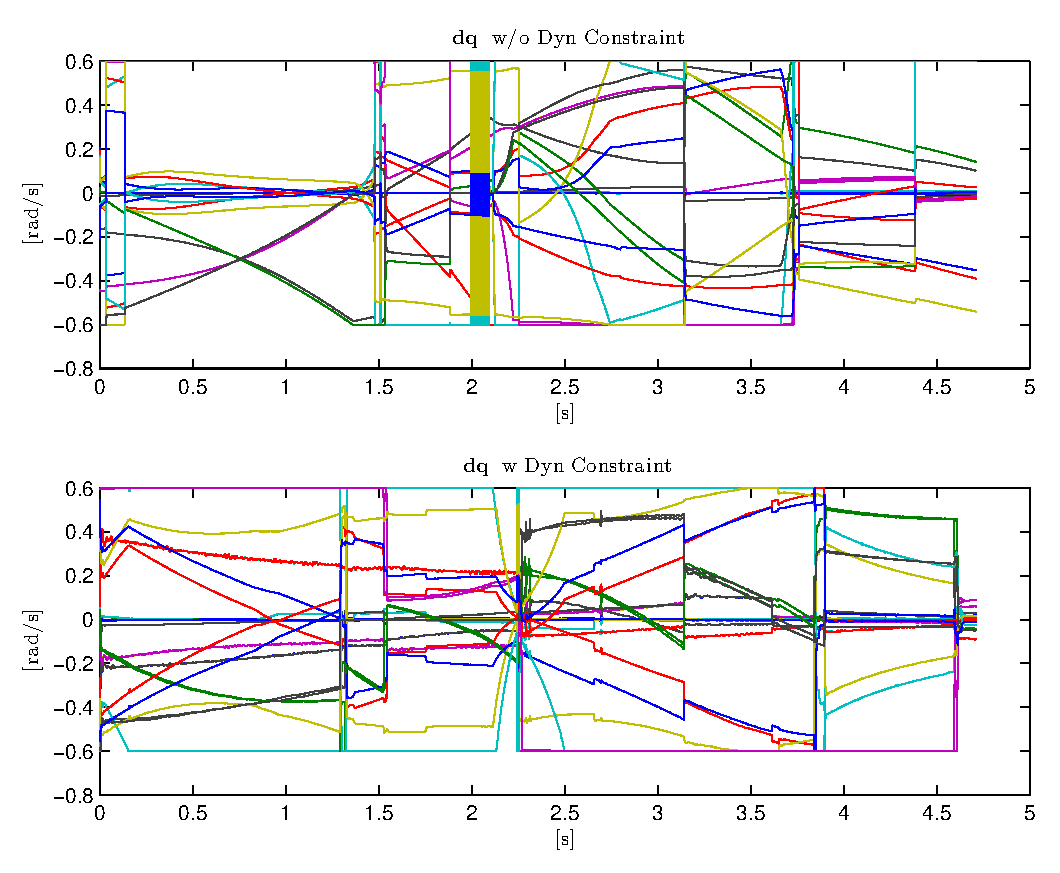
\includegraphics{gfx/dq_dyn.eps} \caption{Computed joint velocities}
        \label{dq_dyn}
    %\end{subfigure}
\end{sidewaysfigure}
\newpage
\begin{sidewaysfigure}
    \centering
    %\begin{subfigure}[b]{0.8\textwidth}
        \includegraphics[width=\textwidth]{gfx/tau_dyn.png}
        %\caption{Dynamics of the Cartesian error}
        %\label{Cartesian_error}
    %\end{subfigure}
    \caption{Computed joint torques}\label{tau_dyn}
\end{sidewaysfigure}
\clearpage